39. $y=\cfrac{(x-1)(x-3)}{|x-2|+1}=\begin{cases} \cfrac{(x-1)(x-3)}{x-2+1},\ x\geqslant2,\\ \cfrac{(x-1)(x-3)}{2-x+1},\ x<2.\end{cases}=
\begin{cases} x-3,\ x\geqslant2,\\ 1-x,\ x<2.\end{cases}$
$$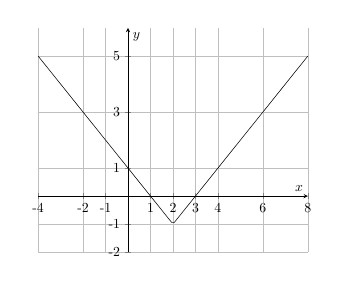
\begin{tikzpicture}[scale=0.5]
\begin{axis}[
    axis lines = middle,
    grid=major,
    legend pos={south west},
    xlabel = {$x$},
    ylabel = {$y$},
    ymin=-2,
    ymax=6,
    xtick={ -4, -1, 1, 4,3, 6,-2,2,8},
    xticklabels={ -4, -1, 1, 4,3, 6,-2,2,8},
    ytick={ -2, 1, -1,3,5},
    yticklabels={ -2, 1, -1,3,5}            ]
	\addplot[domain=-4:8, samples=100, color=black] {(x-1)*(x-3)/(abs(x-2)+1)};
%\addplot[domain=-3.1:2.5, samples=100, color=red] {70*abs(1-2*abs(abs(x)-2))-10*x^2+10*x-70};
	%\addlegendentry{$\text{Рис. 1}$};
\end{axis}
\end{tikzpicture}$$
